% arara: pdflatex

%%%%%%%%%%
%  DRC Abstract Template for LaTeX Users
%  Latest Revision: 11 Jan 2016
%  Author: Samuel James Bader
%
%  README:
%   - This template is provided as a convenience for LaTeX users, and may not
%     suit every user's needs.  Feel free to modify as you see fit, so long as
%     you stay within the rules explicitly given for abstracts.
%   - This template supports both single-column and double-column layouts.
%     You need only change one line to switch, see below under ``IF YOU WANT
%     A TWO-COLUMN LAYOUT.''
%   - This template should work on common LaTeX compilers, but if this fails
%     to compile on your system due to font errors, see below where ``Times
%     New Roman'' is included and try a different one of the given options.
%
%%%%%%%%%%

%%%%%%%%%%
% YOU CAN IGNORE EVERYTHING FROM HERE UNTIL THE \begin{document}
%%%%%%%%%%
\documentclass[10pt]{article}

% Margins must be 1in all around
\usepackage[margin=1in]{geometry}

% Hyperlinks are blue
\usepackage[colorlinks=true, urlcolor=blue]{hyperref}

% URLs don't need to be mono-spaced
\urlstyle{same}

% Short form \email{} for giving email links
\newcommand{\email}[1]{\href{mailto:#1}{\underline{#1}}}

% Get math utilities
\usepackage{amsmath}
\usepackage{amsthm}
\usepackage{amssymb}

% Encodings
\usepackage[T1]{fontenc}
\usepackage[utf8]{inputenc}

% DRC abstracts use the Times New Roman font, and there are
% multiple ways to include this in LaTeX.  Option 1 should work
% for most LaTeX installations; however depending on your set-up,
% you may prefer Option 2 or 3. Uncomment just one option:

% Times New Roman: OPTION 1 (generally recommended)
\usepackage{newtxtext,newtxmath}
\DeclareTextCommandDefault{\textbullet}{\ensuremath{\bullet}}
% Times New Roman: OPTION 2 (fallback for older installations)
%\usepackage{mathptmx}
% Times New Roman: OPTION 3 (for XeLaTeX or LuaLaTeX users)
%\usepackage{fontspec}\setmainfont{Times New Roman}

% Shrink LaTeX line spacing a little to mirror Word template
\usepackage{setspace}
\setstretch{.955}

% Customize the author/affiliation section
\usepackage{authblk}

% No space between author and affiliation lists
\setlength{\affilsep}{0em}

% Authors in font size 12
\renewcommand{\Authfont}{\large}

% Affiliations in font size 10
\renewcommand{\Affilfont}{\itshape\normalsize}

% Define a command for author contact information
% (Wedge it into a ``affiliation'' line with no number.)
\newcommand{\authcontact}[2]{
  \affil[ ]{\textit{Email: \email{#1} / Phone: #2 }}
}

% Customize \maketitle to get rid of extra spacings and enforce font commands
\makeatletter
    \def\@maketitle{%
  \newpage
  \begin{center}%
  \let \footnote \thanks
  {\fontsize{14pt}{16.1pt}\selectfont \textbf{\@title}\par }%
    {\vspace{-3pt}%
      \begin{tabular}[t]{c}%
        \@author
      \end{tabular}\par
    }%
  \end{center}%
  \vspace{-1.2\baselineskip}
}
\makeatother

% Section headers are just bold normal-sized text
\usepackage[tiny]{titlesec}
\titlespacing*{\section}{0em}{\baselineskip}{0em}

% Allow multiple columns
\usepackage{multicol}
\setlength{\columnsep}{.5em}
\newif\ifdoublecol\doublecolfalse

% No numbered page footer
\pagestyle{empty}

% Keep numbered/bulleted lists compact
\usepackage{enumitem}
\setlist{nosep}

% Figures
\usepackage{graphicx}
\usepackage{svg}

% Label with Fig rather than figure.
\renewcommand{\figurename}{Fig.}

% Reduce line spacing in the bibliography
\usepackage{etoolbox}
\apptocmd{\thebibliography}{\setlength{\itemsep}{0em}}{}{}

%%%%%%%%%%
% START PAYING ATTENTION NOW
%%%%%%%%%%
\begin{document}

% IF YOU WANT A TWO-COLUMN LAYOUT, uncomment the following line
%\doublecoltrue

% Your TITLE goes here:
\title{Design and optimization of the phase-transition FET}

% AUTHOR LIST, with numbers indicating affiliation
\author[1]{Samuel James Bader}
\author[2]{Debdeep Jena}

% AFFILIATION LIST, with numbers to match the author list
\affil[1]{Department of Applied Physics, Cornell University, Ithaca, NY}
\affil[2]{Departments of ECE and MSE, Cornell University, Ithaca, NY}

% AUTHOR CONTACT INFORMATION here: email and phone number.
\authcontact{sjb353@cornell.edu}{(607)-255-1450 [Asst.]}
\maketitle
\thispagestyle{empty}

% Makes a double column layout *if specified above*
\ifdoublecol\begin{multicols}{2}\fi

% YOUR TEXT HERE
\section*{Introduction}
As the juggernaut of CMOS scaling collides with the thermodynamic limits of subthreshold swing, researchers in recent years have pursued numerous classes of devices incorporating additional physics, such as interband tunneling, ferroelectricity, nano-mechanics, band-modulation, and resistive switching materials \cite{Cristoloveanu_2016}.  One such scheme from the latter category, termed the \textit{Hybrid Phase-transition FET} (or \textit{HyperFET}), simply incorporates a resistive switching material in the source of an otherwise standard transistor \cite{Shukla_2015} as depicted in Figure \ref{fig:HyperFETConstruction}c.  This phase-change resistor impedes low currents, but yields to high currents, providing a steepness boost to a Boltzmann-limited transistor.

Rapid progress in this field has demonstrated devices with local subthreshold slopes tighter than 8mV/decade at room temperature, leading to $I_\mathrm{ON}$ enhancement of more than a third \cite{Frougier_2016}, and researchers have demonstrated sub-nanosecond switching \cite{Frougier_2016,Jerry_2016} of relatively large devices, with projections of much faster switching times for more aggressively scaled devices \cite{Jerry_2016}.  In addition to experimental advances, authors have projected the scaling requirements of these devices based on circuit simulation with predicted values of various nodes \cite{Shukla_2015,Frougier_2016}. 

\section*{New Contributions}
While circuit simulation gives accurate predictions when inputs are well-characterized, direct mathematical analysis provides a separate dimension of insight with clear identification of precisely which features a prediction depends upon. And given the simplicity of the resistive-source transistor ``circuit'', this device lends itself to a straightforward and illuminating analysis.

This work employs a simple, generic, analytic short-channel transistor model \cite{Khakifirooz_2009}.  This model was originally proposed for scaled Si CMOS devices but has been successfully adapted to other material systems, and its small physical parameter set enables both direct analytic work and quick fitting to projections.  This model is combined with the simplest possible phase-change resistor model: a single piecewise linear, discontinuous and potentially hysteretic expression.  Given the elementary nature of the expressions involved, compact solutions for several regimes of the HyperFET I-V curve can be derived in short-order.

With these expressions in hand, one can make numerous statements about HyperFETs without recourse to simulation.  The subthreshold and inversion behavior are derived, as well as the width and positioning of the hysteresis under relatively general conditions.  A procedure of threshold-shifting the HyperFET to match its off-current to that of the isolated transistor (as employed numerically in \cite{Shukla_2015, Frougier_2016}) is carried out analytically, and this is used to derive simple expressions for the ``shifting'' gain provided by the phase-change resistor. 

From there, the dependence of the shifting gain on various material and geometry parameters emerges, and optimization of this gain with respect to resistor scaling is discussed analytically.  The condition for above-unity gain, as approached by simulation in \cite{Frougier_2016}, is clearly derived and intuitively stated.  Approximations to the optimal resistor geometry from a DC I-V perspective are derived under given safety margins on the hysteresis boundaries.

\section*{Significance}
The mathematics provided in this work unifies numerous statements about HyperFET scaling -- which have until now depended on simulations -- into an intuitive, analytical framework, clarifying the relative importances and influences of various parameters bearing on the device characteristics.  These formulae should be of use to benchmarkers seeking the best parameter ranges to compare. And the optimization procedures described herein should aid researchers in the choice of experimental parameters as HyperFET demonstration continues to scale to more and more challenging dimensions.

% END YOUR TEXT

% Closes the double-column layout *if specified above*
\ifdoublecol\end{multicols}\fi

% Skip to bottom of page
\vfill

% Start double-column for References, 9pt font
\setlength{\multicolsep}{0em}
\begin{multicols}{2}
{\fontsize{9pt}{9pt}\selectfont

% Prevent extra spaces following periods in bibliography
\frenchspacing

% Prevents the bibliography from being titled
\renewcommand{\section}[2]{}
\begin{thebibliography}{9} 

% YOUR REFERENCES HERE
\bibitem{Cristoloveanu_2016} 
Cristoloveanu et al.  IEEE EDS, 4(5), 215 (2016)
\bibitem{Shukla_2015}
Shukla et al. Nature comm. 6, 7812 (2015)
\bibitem{Frougier_2016}
Frougier et al. Symposium on VLSI Technology, IEEE 2016
\bibitem{Jerry_2016}
Jerry et al. Silicon Nanoelectronics Workshop, IEEE 2016
\bibitem{Khakifirooz_2009}
Khakifirooz et al.  IEEE Trans. Elec. Dev. 56(8), 1674 (2009)
% END YOUR REFERENCES

% Done with bibliography
\end{thebibliography}
}
\end{multicols}

% Now Figures Page
\pagebreak

\begin{figure}[!ht]
  \centering
  %\includesvg[width=\textwidth, svgpath=images/]{HyperFETConstruction}
  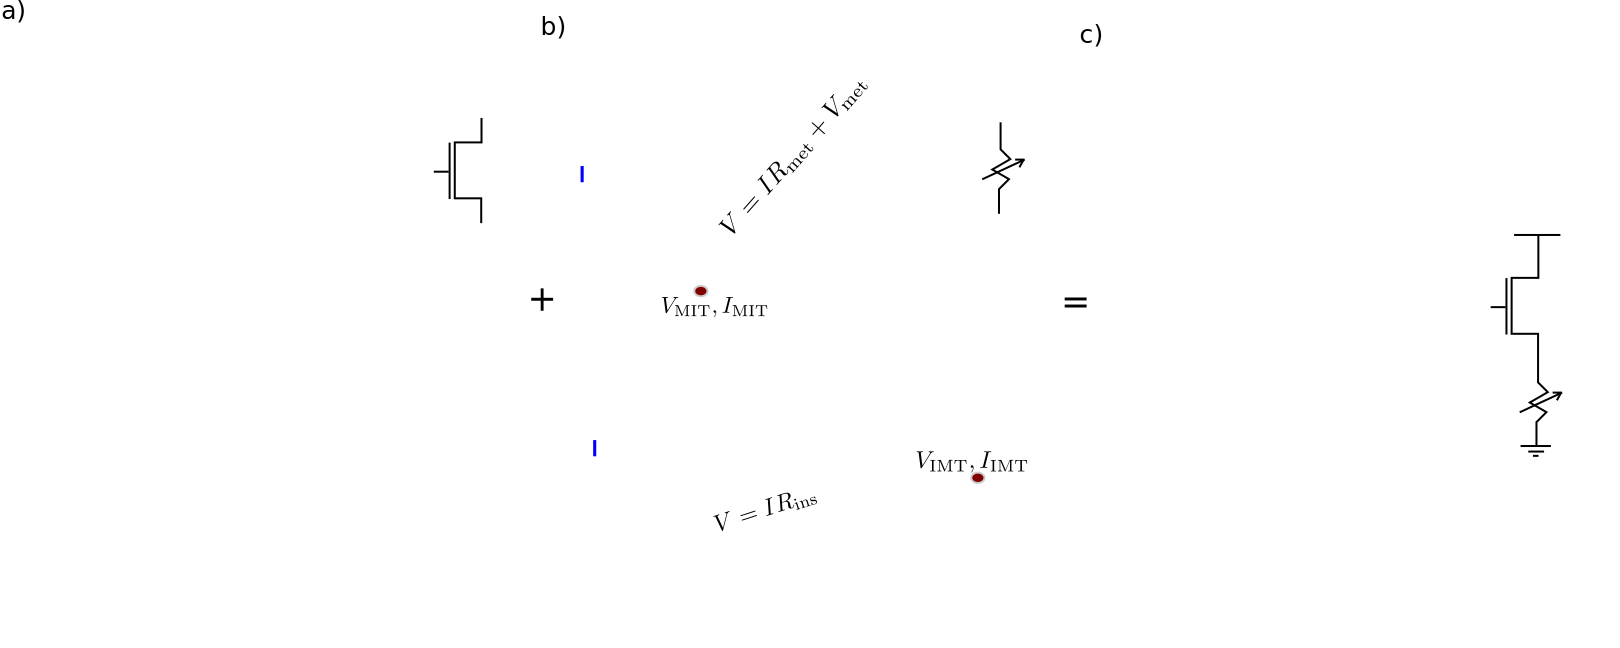
\includegraphics[width=\textwidth]{images/HyperFETConstruction}
  \caption{Some caption}
  \label{fig:HyperFETConstruction}
\end{figure}
\begin{figure}[!ht]
  \centering
  %\includesvg[width=\textwidth, svgpath=images/]{HyperFETConstruction}
  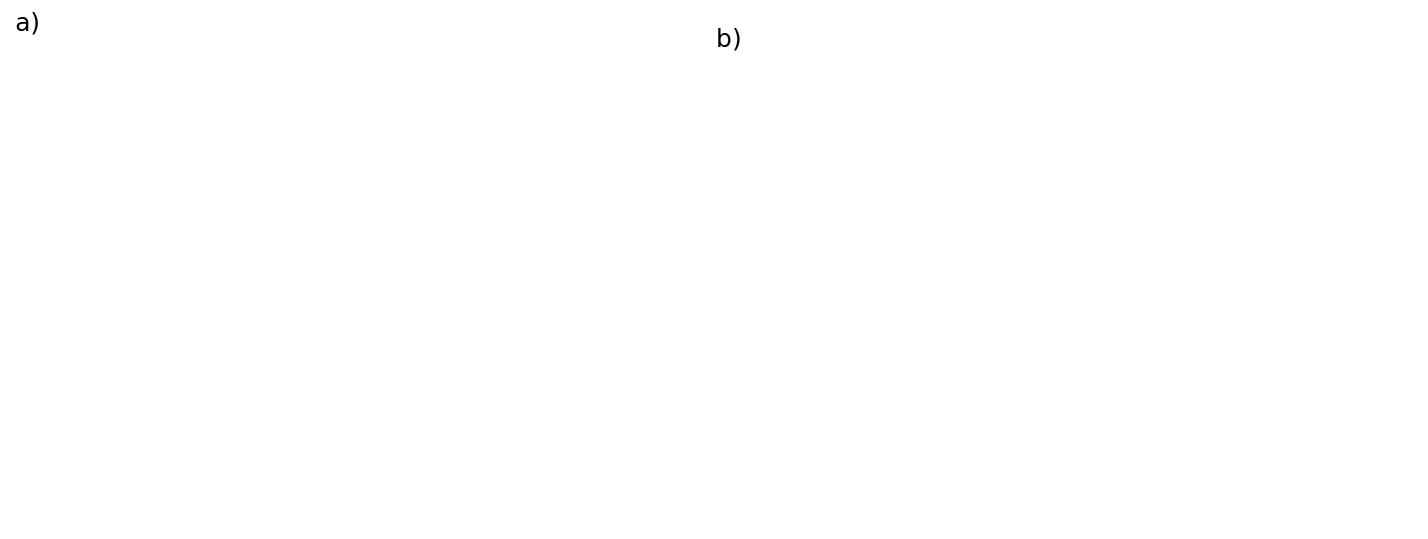
\includegraphics[width=\textwidth]{images/HFvsGeo}
  \caption{Some caption}
  \label{fig:HFvsGeo}
\end{figure}


% A figure containing two graphics in minipages
%\begin{figure}[!ht]
%  \centering
%  \begin{minipage}[t]{.49\textwidth}
%    \includegraphics[width=\textwidth]{images/Fig1}
%    \caption{This is an example figure to show one method for creating the figures on this page.  Two minipages just smaller than half the pagewidth are placed in one ``figure'' environment.  Each minipage holds one graphic/caption, and the two are horizontally stacked.}
%    \label{fig:CNT}
%  \end{minipage}
%\hfill
%  \begin{minipage}[t]{.49\textwidth}
%    \includegraphics[width=\textwidth]{images/Fig2}
%    \caption{Of course, seeing as this \textit{is} LaTeX, there are many different methods you could use for placing/aligning figures if you want to get more precise.  For starters, check out  \url{http://tex.stackexchange.com/a/148445/39047} or \url{https://en.wikibooks.org/wiki/LaTeX/Floats,_Figures_and_Captions}.}
%    \label{fig:channel}
%  \end{minipage}
%\end{figure}

% A plain old figure
%\begin{figure}[!ht]
%  \centering
%    \includegraphics[width=\textwidth]{images/Fig3}
%    \caption{Of course, you don't have to get fancy.  Here's a basic figure just spanning the width of the page.  But do notice the individually labelled subparts, and the fact that there is no more text on this page beyond captions.}
%    \label{fig:length}
%\end{figure}


% Thank you for your abstract!
\end{document}
